\section{Reclaiming space}
\label{sec:space}

Copy-on-write never overwrites a page, so every checkpoint leaves behind the images it replaced. They stay reachable while a retained generation refers to them and become garbage afterwards. Segments are append-only, so garbage is never reused piece by piece: HStore copies the live images out of mostly dead segments and deletes the files. This needs two things, knowing which images are live and moving them without touching the trees that point at them.

\subsection{Reference counts between checkpoints}

Every page number has a reference count in a memory-mapped file laid out like the directory. The count is the number of places that point at the page in the last checkpointed generation: a slot root, a child reference in a branch, or a nested tree's root inside a record. Inline trees have no page and are never counted. A negative entry marks a page that died in generation $d$ and is waiting until no reader can see a generation older than $d$.

Counts change only at checkpoints, and only between two generations whose trees are fully written: the one the previous checkpoint wrote and the one the current checkpoint just wrote. Generations published in between are never counted. Their new nodes have no pages, and every page they reach was counted by the previous checkpoint or is \emph{provisional} (spilled by a bulk load or written by a large commit, and resolved by the checkpoint that covers it). For each branch whose roots changed, the counter first adds one to every new root, recursing into a page only when its count rises from zero, and then subtracts one from every old root, recursing only when a count reaches zero. When a node is replaced, its children are added by the new copy and subtracted by the old one, so they cancel and are never touched. The work is proportional to the pages that changed between the two checkpoints, not to the number of commits or the size of the trees. Most of the nodes it reads are in the node cache because the checkpoint has just written them. A header flag records whether a leaf refers to any page, so leaves that hold only plain records or inline trees, such as most catalog leaves, are never decoded.

A page that died in generation $d$ is released at a checkpoint once $d$ is no newer than the oldest generation anyone can still read, the older of the oldest retained and the oldest pinned generation. Releasing clears its directory entry and subtracts its bytes from its segment's live total. The changed counts and the cleared entries are journaled with absolute values before the catalog image is published and applied afterwards, so a crash leaves the files as of one checkpoint or the next, never a mix, and applying a journal twice is harmless.

\begin{figure}[t]
\centering
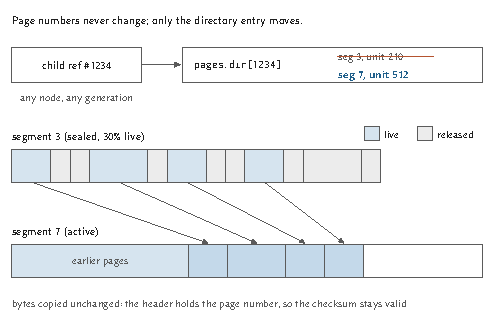
\includegraphics[width=\columnwidth]{figures/compaction}
\caption{Compaction copies the live images of a mostly dead segment to the active segment and changes their directory entries. Every tree, in every generation and branch, still refers to the same page numbers.}
\label{fig:compaction}
\end{figure}

\subsection{Compaction by moving}

A sealed segment whose live bytes fall below a threshold (half of the bytes written to it, by default) is a compaction victim. Compaction reads through the victim one 64-byte unit at a time (\cref{fig:compaction}). Where a header starts and the directory entry for that header's page number points at exactly this place, the image is live: it is verified and its bytes are appended to the active segment. Anything else, such as a released image or an older copy of a moved one, is skipped. The header holds the page number, not the address, so neither the header nor the checksum changes. After every 4\,MiB of copies the segments are forced, and only then are the directory entries pointed at the copies, so an entry never reaches the disk ahead of the bytes it points to. The victim is then retired, and its file is deleted after the next checkpoint has made the new entries durable and once no pinned reader started before the move.

Nothing in this takes the commit lock or commits anything. Commits continue while pages move, cached nodes stay valid because they are keyed by page number, and old generations reach the moved pages through the same directory, so compaction never shortens the time-travel window. Moves are not logged. If the engine crashes before the checkpoint that follows a compaction, recovery restores the directory entries of the replayed commits to their original addresses, which are still intact because victims are deleted only after that checkpoint. The copies become unreferenced space that a later pass reclaims. The work is proportional to the size of the victims, and the only memory it needs is the list of pages moved in the current 4\,MiB.

A background pass compacts the emptiest victim every 500\,ms if one exists; an explicit request compacts all of them. A new segment gets 8\,MiB, doubled as long as it stays within an eighth of the bytes in the other segments, up to 256\,MiB. A small database therefore has several sealed segments for compaction to choose from, and a large one has few files. The engine keeps at most 256 segment files open and closes the least recently used one, after forcing it if it has unsynced writes, so the number of open files does not grow with the database.
